\documentclass[journal,12pt,twocolumn]{IEEEtran}
%
\usepackage{setspace}
\usepackage{gensymb}
%\doublespacing
\singlespacing

\usepackage{graphicx}
\usepackage[cmex10]{amsmath}
\usepackage{amsmath,amsthm}
\usepackage{mathrsfs}
\usepackage{txfonts}
\usepackage{stfloats}
\usepackage{bm}
\usepackage{cite}
\usepackage{cases}
\usepackage{subfig}

\usepackage{longtable}
\usepackage{multirow}
\usepackage{commath}
\usepackage{enumitem}
\usepackage{mathtools}
\usepackage{steinmetz}
\usepackage{tikz}
\usepackage{circuitikz}
\usepackage{verbatim}
\usepackage{tfrupee}
\usepackage[breaklinks=true]{hyperref}

\usepackage{tkz-euclide}

\usetikzlibrary{calc,math}
\usepackage{listings}
    \usepackage{color}                                            
    \usepackage{array}                                            
    \usepackage{longtable}                                        
    \usepackage{calc}                                             
    \usepackage{multirow}                                         
    \usepackage{hhline}                                           
    \usepackage{ifthen}                                           
    \usepackage{lscape}     
\usepackage{multicol}
\usepackage{chngcntr}

\DeclareMathOperator*{\Res}{Res}

\renewcommand\thesection{\arabic{section}}
\renewcommand\thesubsection{\thesection.\arabic{subsection}}
\renewcommand\thesubsubsection{\thesubsection.\arabic{subsubsection}}

\renewcommand\thesectiondis{\arabic{section}}
\renewcommand\thesubsectiondis{\thesectiondis.\arabic{subsection}}
\renewcommand\thesubsubsectiondis{\thesubsectiondis.\arabic{subsubsection}}

\hyphenation{op-tical net-works semi-conduc-tor}
\def\inputGnumericTable{}                                 

\lstset{
%language=C,
frame=single, 
breaklines=true,
columns=fullflexible
}
\lstset{
%language=TeX,
frame=single, 
breaklines=true
}

\begin{document}

\newtheorem{theorem}{Theorem}[section]
\newtheorem{problem}{Problem}
\newtheorem{proposition}{Proposition}[section]
\newtheorem{lemma}{Lemma}[section]
\newtheorem{corollary}[theorem]{Corollary}
\newtheorem{example}{Example}[section]
\newtheorem{definition}[problem]{Definition}

\newcommand{\BEQA}{\begin{eqnarray}}
\newcommand{\EEQA}{\end{eqnarray}}
\newcommand{\define}{\stackrel{\triangle}{=}}
\bibliographystyle{IEEEtran}
\providecommand{\mbf}{\mathbf}
\providecommand{\pr}[1]{\ensuremath{\Pr\left(#1\right)}}
\providecommand{\qfunc}[1]{\ensuremath{Q\left(#1\right)}}
\providecommand{\sbrak}[1]{\ensuremath{{}\left[#1\right]}}
\providecommand{\lsbrak}[1]{\ensuremath{{}\left[#1\right.}}
\providecommand{\rsbrak}[1]{\ensuremath{{}\left.#1\right]}}
\providecommand{\brak}[1]{\ensuremath{\left(#1\right)}}
\providecommand{\lbrak}[1]{\ensuremath{\left(#1\right.}}
\providecommand{\rbrak}[1]{\ensuremath{\left.#1\right)}}
\providecommand{\cbrak}[1]{\ensuremath{\left\{#1\right\}}}
\providecommand{\lcbrak}[1]{\ensuremath{\left\{#1\right.}}
\providecommand{\rcbrak}[1]{\ensuremath{\left.#1\right\}}}
\theoremstyle{remark}
\newtheorem{rem}{Remark}
\newcommand{\sgn}{\mathop{\mathrm{sgn}}}
\providecommand{\abs}[1]{\(\left\vert#1\right\vert\)}
\providecommand{\res}[1]{\Res\displaylimits_{#1}} 
\providecommand{\norm}[1]{\(\left\lVert#1\right\rVert\)}
%\providecommand{\norm}[1]{\lVert#1\rVert}
\providecommand{\mtx}[1]{\mathbf{#1}}
\providecommand{\mean}[1]{E\(\left[ #1 \right]\)}
\providecommand{\fourier}{\overset{\mathcal{F}}{ \rightleftharpoons}}
%\providecommand{\hilbert}{\overset{\mathcal{H}}{ \rightleftharpoons}}
\providecommand{\system}{\overset{\mathcal{H}}{ \longleftrightarrow}}
	%\newcommand{\solution}[2]{\textbf{Solution:}{#1}}
\newcommand{\solution}{\noindent \textbf{Solution: }}
\newcommand{\cosec}{\,\text{cosec}\,}
\providecommand{\dec}[2]{\ensuremath{\overset{#1}{\underset{#2}{\gtrless}}}}
\newcommand{\myvec}[1]{\ensuremath{\begin{pmatrix}#1\end{pmatrix}}}
\newcommand{\mydet}[1]{\ensuremath{\begin{vmatrix}#1\end{vmatrix}}}
%\numberwithin{equation}{section}
\numberwithin{equation}{subsection}
%\numberwithin{problem}{section}
%\numberwithin{definition}{section}
\makeatletter
\@addtoreset{figure}{problem}
\makeatother
\let\StandardTheFigure\thefigure
\let\vec\mathbf
%\renewcommand{\thefigure}{\theproblem.\arabic{figure}}
\renewcommand{\thefigure}{\theproblem}
%\setlist[enumerate,1]{before=\renewcommand\theequation{\theenumi.\arabic{equation}}
%\counterwithin{equation}{enumi}
%\renewcommand{\theequation}{\arabic{subsection}.\arabic{equation}}
\def\putbox#1#2#3{\makebox[0in][l]{\makebox[#1][l]{}\raisebox{\baselineskip}[0in][0in]{\raisebox{#2}[0in][0in]{#3}}}}
     \def\rightbox#1{\makebox[0in][r]{#1}}
     \def\centbox#1{\makebox[0in]{#1}}
     \def\topbox#1{\raisebox{-\baselineskip}[0in][0in]{#1}}
     \def\midbox#1{\raisebox{-0.5\baselineskip}[0in][0in]{#1}}
\vspace{3cm}
\title{Assignment 1}
\author{Vishal Ashok}
\maketitle
\newpage
%\tableofcontents
\bigskip
\renewcommand{\thefigure}{\theenumi}
\renewcommand{\thetable}{\theenumi}
\begin{abstract}
This document explains how to find the point of intersection of a line and a plane.
\end{abstract}
Download the python code from 
%
\begin{lstlisting}
https://github.com/vishalashok98/AI5006/tree/master/Assignment1
\end{lstlisting}
%
and latex-tikz codes from 
%
\begin{lstlisting}
https://github.com/vishalashok98/AI5006/tree/master/Assignment1
\end{lstlisting}
%

\section{Problem}
Find the co ordinates of the point when the line through
\myvec{3\\-4\\-5} and \myvec{1\\-3\\1} crosses the plane [2  1  1]x=7 and perpendicular to the two lines

	
	
\section{Explanation}
Equation of a line passing through the point \myvec{3\\-4\\-5} and \myvec{1\\-3\\1} is given by:
\begin{center}

$\frac{x-3}{2} = \frac{y+4}{-1}= \frac{z+5}{-6}$ \label{eq:1}
\end{center}

A line can be considered as intersection of two planes ,from equation 1 equations of two planes can be given as
\begin{center}
$\frac{x-3}{2} = \frac{y+4}{-1}$\label{eq:2}
\end{center}

and
\begin{center}
$\frac{x-3}{2} = \frac{y+4}{-1}$\label{eq:3}
\end{center}
So there are three set of equations which should be solved to find the point of intersection.





\section{Solution}
There are three equations 
\begin{align}
2x+y+z=7\label{eq:1}
\end{align}
\begin{align}
x+2y+0=-5    \label{eq:2}
\end{align}
    
\begin{align}
3x+0+z=8\label{eq:3}
\end{align}

These equations can be represented in matrix form as

\begin{align}
\myvec{2 & 1 & 1 \\ 1 & 2 & 0\\3 & 0 &1}\myvec{x\\y\\z}=\myvec{7\\-5\\8}
\end{align}	
Writing it in the form of augumented matrix and reducing it to echolon form we get

\begin{align}
\myvec{2 & 1 & 1 & :& 7\\ 1 & 2 & 0 & : & -5\\3 & 0 & 1 & : & 8} \xleftrightarrow{R_2=R_2-R_1/2}\myvec{2 & 1 & 1 & : & 7\\0 & 1.5 & -0.5 & : & -8.5\\ 3 & 0 & 1 & : & 8 }	
\end{align}


\begin{align}
\myvec{2 & 1 & 1 & : & 7\\0 & 1.5 & -0.5 & : & -8.5\\ 3 & 0 & 1 & : & 8 }\xleftrightarrow{R_3=R_3-1.5R_1}\myvec{2 & 1 & 1 & : & 7\\0 & 1.5 & -0.5 & : & -8.5\\ 0.5 & -1.5 & -0.5 & : & -2.5 }    
\end{align}

\begin{align}
\myvec{2 & 1 & 1 & : & 7\\0 & 1.5 & -0.5 & : & -8.5\\ 0.5 & -1.5 & -0.5 & : & -2.5 }\xleftrightarrow{R_3=R_3+R_2}\myvec{2 & 1 & 1 & : & 7\\0 & 1.5 & -0.5 & : & -8.5\\ 0 & 0 & -1 & : & -11 }
\end{align}

\begin{align}
\myvec{2 & 1 & 1 & : & 7\\0 & 1.5 & -0.5 & : & -8.5\\ 0 & 0 & -1 & : & -11 }\xleftrightarrow{R_2=R_2+0.5R_3}\myvec{2 & 1 & 1 & : & 7\\0 & 1.5 & 0 & : & -3\\ 0 & 0 & -1 & : & -11 }
\end{align}

\begin{align}
\myvec{2&1&1&:&7\\0&1.5&0&:&-3\\0&0&-1&:&-11 }\xleftrightarrow{R_1=R_1+R_3-0.666R_2}\myvec{2&0&0&:&-2\\0&1.5&0&:&-3\\ 0&0&-1&:&-11}
\end{align}    


So from the Row reduced echolon form of matrix we know that point of intersection is $[-1,-2,11]$

\section{Plot}
\begin{figure}[!htbp]
    \centering
    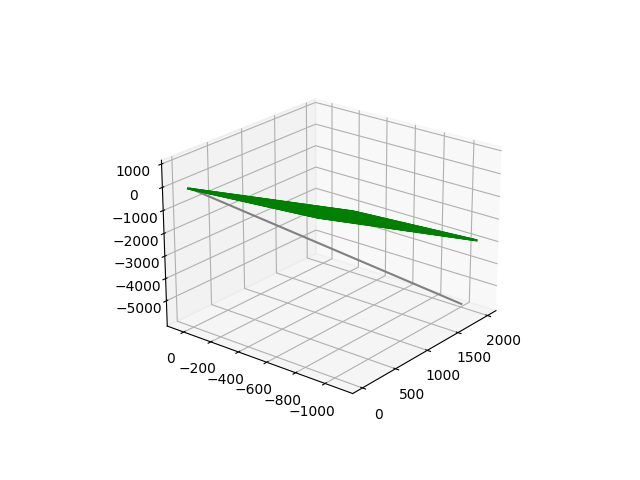
\includegraphics[width =\columnwidth]{Figure_1.png}
    \caption{Intersection of Plane and Line }
    \label{fig:1}
\end{figure}
\end{document}
